\section{A universal exact common-radius certificate}
\label{sec:radius}
The fixed-radius antichain answers many failure rules at one geometry. This section fixes the sites and target and determines the exact common radius needed for any one of those rules. All sites share the same radius in this theorem. Unequal-radius targets are handled by \cref{thm:sweep}, but the bisector proof below must not be applied unchanged to additive weighted distances.

Let $w:2^{[n]}\to\{0,1\}$ be monotone, with $w(\varnothing)=0$ and $w([n])=1$. Define
\begin{equation}\label{eq:required-radius}
\rho_w(x)=\min_{\sigma:\,w(\sigma)=1}\max_{i\in\sigma}\|x-c_i\|.
\end{equation}
This is the smallest common radius for which the active contact set at $x$ wins. It is a finite minimum of finite maxima of distance functions, so it is continuous and $1$-Lipschitz. The same maximum--minimum algebra underlies lattice-polynomial descriptions of reliability systems~\cite{lattice,reliability-lattice}.

\begin{lemma}[Prefix evaluation]\label{lem:prefix}
Order the squared site distances at $x$, adding every tied group together. The first prefix on which $w$ wins has maximum squared distance $\rho_w(x)^2$.
\end{lemma}
\begin{proof}
At squared radius $s$, the active set is exactly the union of all distance groups at most $s$. Before its first winning prefix, no winning subset can be contained in that active set. At the first winning prefix, the prefix itself is a winning coalition. This is exactly the minimization in \cref{eq:required-radius}.
\end{proof}

Let $\mathscr L$ contain all nontrivial perpendicular bisectors of pairs of sites and the supporting lines of all target edges. Coincident sites give no bisector; coincident lines are stored once. Let $Q_T$ contain all target vertices and every intersection of two nonparallel lines in $\mathscr L$ that lies in $T$.

\begin{theorem}[An elementary arrangement certificate]\label{thm:master-radius}
For rational sites and a triangular target,
\begin{equation}\label{eq:master-radius}
r_w^*:=\min\{r\ge0:T\subseteq R_w(r)\}
=\max_{q\in Q_T}\rho_w(q).
\end{equation}
The candidate set $Q_T$ is independent of $w$, has rational coordinates and has at most $O((n^2+h)^2)$ points. In particular $(r_w^*)^2\in\mathbb Q$. A maximizing point is an exact target witness showing that every smaller common radius fails.
\end{theorem}
\begin{proof}
The perpendicular bisectors divide the plane into cells on which the weak ordering of distances to the sites is fixed. Identical sites remain tied everywhere; there is no need to break such a tie geometrically. The additional target-edge lines subdivide every target triangle into bounded convex polygons. On the interior of one such polygon, \cref{lem:prefix} selects one fixed distance group, so $\rho_w(x)$ equals $\|x-c_j\|$ for a fixed representative site $c_j$ in that group.

The norm function is convex. Every point of the polygon is a convex combination of its vertices, and its distance to $c_j$ is at most the corresponding convex combination of vertex distances. Thus the maximum on the polygon is attained at a vertex. By continuity of $\rho_w$, the formula obtained in its interior extends to its boundary even when new distance ties occur there. Every polygon vertex is either a target vertex or an intersection of two lines in $\mathscr L$, hence belongs to $Q_T$. Taking the maximum over the finitely many target polygons proves that $\max_T\rho_w=\max_{Q_T}\rho_w$.

Coverage at common radius $r$ is equivalent to $r\ge\rho_w(x)$ at every target point by definition, giving \cref{eq:master-radius}. There are at most $\binom n2+h$ lines and a quadratic number of their pairwise intersections. Rational line coefficients give rational intersection coordinates. Squared distances at those points are rational, and \cref{lem:prefix} selects one of them. Their finite maximum is rational. A maximizing point fails at any smaller radius, proving the witness assertion.
\end{proof}

\begin{remark}[Universality and complexity]
The same $Q_T$ works for cardinality thresholds, weighted budgets, domain rules and any fixed monotone activation of primitive contacts. It does not say that the critical radius is the same for those rules. Its point is reusability and an exact threshold; specialised higher-order or coloured Voronoi methods can be faster for a single rule.
\end{remark}

\subsection{The support reduction in fixed dimension}
The full line arrangement contains many vertices created by distance ties that are irrelevant to a given threshold. A local maximum argument removes them simultaneously for every monotone rule. We state the argument in $\R^d$ to make the supporting geometry explicit.

For a finite union of rational nondegenerate $d$-simplices, construct a set $Q_T^{\mathrm{supp}}$ as follows. Include every simplex vertex. For each $f$-dimensional face $G$ of each simplex, with $1\le f\le d$, and each choice of $f+1$ sites, solve the $f$ equations asserting equal squared distance to those sites, restricted to the affine hull of $G$. Retain the solution if it is unique and lies in $G$. All these equations are linear after subtracting one squared-distance equation from the others.

\begin{theorem}[Universal support certificate]\label{thm:support-radius}
For every monotone rule $w$ with $w(\varnothing)=0$ and $w([n])=1$,
\begin{equation}\label{eq:support-radius}
r_w^*=\max_{q\in Q_T^{\mathrm{supp}}}\rho_w(q).
\end{equation}
The set is independent of $w$, has rational coordinates, and for $t$ supplied simplices has size at most
\begin{equation}\label{eq:support-count}
t(d+1)+t\sum_{f=1}^d\binom{d+1}{f+1}\binom n{f+1}.
\end{equation}
In particular, for fixed dimension it has $O(t(1+n^{d+1}))$ points, and $(r_w^*)^2$ is rational.
\end{theorem}
\begin{proof}
Choose a maximizer $x$ of the continuous function $\rho_w$ on $T$. Choose one target simplex containing $x$, and let $G$ be its unique face whose relative interior contains $x$. Write $f=\dim G$. If $f=0$, $x$ is a supplied vertex and is already in the certificate.

Suppose $f\ge1$. Let $s=\rho_w(x)$, let $L$ contain the sites strictly closer than $s$, and let $J$ contain those at distance exactly $s$. By \cref{lem:prefix}, $w(L)=0$ and $w(L\cup J)=1$. There is a neighborhood of $x$ in which all sites of $L$ remain closer than all sites of $J$, and all other sites remain farther than all sites of $J$.

Fix $j_0\in J$. Consider the linear functionals $v\mapsto(c_j-c_{j_0})\cdot v$ on the $f$-dimensional tangent space of $G$. If they have rank less than $f$, choose a nonzero tangent vector $v$ annihilated by all of them. Along $x+uv$ all distances to sites in $J$ remain equal: their squared-distance differences are zero at $u=0$ and have zero linear coefficient. For sufficiently small positive and negative $u$, the order separation from $L$ and the farther sites persists, and $x+uv$ stays in $G$. The winning threshold is therefore the common distance to $J$.

Its square along this line is
\[
\|x+uv-c_{j_0}\|^2
=s^2+2u\,v\cdot(x-c_{j_0})+u^2\|v\|^2.
\]
Since $v\ne0$, at least one of two sufficiently small opposite nonzero values of $u$ makes this strictly larger than $s^2$. This contradicts maximality of $x$.

The functionals thus have rank $f$. Choose $f$ independent ones, corresponding to $f$ sites in $J$ together with $j_0$. Their equal-distance equations have a unique solution in the affine hull of $G$, namely $x$. This is one of the retained support points. Consequently a global maximizer lies in the certificate, proving \cref{eq:support-radius}. The count enumerates the faces and site subsets; singular systems can only reduce it. Unique solutions of rational linear systems are rational, and \cref{lem:prefix} again makes the squared threshold rational.
\end{proof}

\begin{corollary}[Three-site planar construction]\label{cor:three-site}
In the plane it suffices to retain target vertices, intersections of site-pair bisectors with target-edge segments, and circumcenters of noncollinear site triples that lie in the target. The size is $O(n^3+n^2h+h)$.
\end{corollary}
\begin{proof}
The $f=1$ systems are bisector--edge intersections; a bisector coinciding with an edge does not have full rank and contributes no isolated solution. The $f=2$ systems are the circumcenters of noncollinear triples. There are at most $\binom n2$ bisectors and $h$ edges, at most $\binom n3$ circumcenters and $O(h)$ supplied vertices.
\end{proof}

The full arrangement construction provides a second analytical construction of a valid support set. The support theorem gives the smaller main construction. Its proof treats arbitrary monotone rules, not only the $k$th-nearest distance.

\begin{corollary}[One support set for every common radius]\label{cor:all-radii}
For each $r\ge0$,
\begin{equation}\label{eq:antichain-support}
\mathcal A_T(r)=\Min\{S_r(q):q\in Q_T^{\mathrm{supp}}\}.
\end{equation}
Thus a single rational support set recovers the exact target antichain at every common radius and answers every monotone failure query there. The same statement holds after a monotone activation map.
\end{corollary}
\begin{proof}
For any downward-closed family $\F$, let $w$ be its complement. If $w([n])=0$, no contact set can win and both the target and the support set fail. Otherwise \cref{thm:support-radius} says that winning at all support points at radius $r$ is equivalent to winning throughout $T$. The two collections of realized masks therefore have identical answers to every failure-family query. Their minimal antichains must coincide: if a true minimal pattern $A$ had no sampled pattern contained in it, the query $\F=2^A$ would accept all samples and fail at $A$. Conversely every sampled mask is realized in $T$ and contains a true minimal pattern. This proves \cref{eq:antichain-support}. Composition with an activation map preserves monotonicity, giving the last assertion.
\end{proof}

Support witnesses can lie on the target boundary. The vertical algorithm instead supplies interior witnesses for the same minimal masks. Either is a valid rational target witness; their roles must not be confused with merely checking a finite grid chosen without a completeness theorem.

\subsection{Exact line arithmetic}
The bisector of $c_i$ and $c_j$ is
\[
2(c_j-c_i)\cdot x+\|c_i\|^2-\|c_j\|^2=0.
\]
Represent a line by its rational coefficients $(a,b,c)$ in $ax+by+c=0$. Clearing denominators, dividing by the common integer divisor and choosing the first nonzero coefficient positive gives a canonical representation. For two lines $(a,b,c)$ and $(d,e,f)$ with determinant $\Delta=ae-db\ne0$, their intersection is
\[
x=\frac{bf-ec}{\Delta},\qquad y=\frac{cd-fa}{\Delta}.
\]
Every candidate membership test in a closed triangle is a rational orientation test. Every distance-prefix comparison uses rational squared distances. Consequently the radius computation uses no radical comparison; radicals appear only when displaying the final radius as $\sqrt s$.

\subsection{A reusable engineering example}
Take the four sites $(\pm1,\pm1)$ and target $[-3/5,3/5]^2$. Two-contact coverage requires squared radius $68/25$. Assigning both contacts in each column to the same failure domain requires squared radius $89/25$ to survive a domain loss. Assigning the two diagonals as the domains instead requires $68/25$. The saved rational worst points include $(-3/5,0)$ for column wiring and a target corner for diagonal wiring.

These values are derived directly in \cref{app:worked}. The separation is operational: a nominal radius $9/5$ lies between the two thresholds. At that radius, diagonal wiring meets the one-domain-loss requirement and column wiring fails, although ordinary two-contact coverage is identical in both designs.

\subsection{Why unequal offsets require a different proof}
If contact $i$ has radius $r_i+s$ with a common additive design variable $s$, the relevant scalar functions are $\|x-c_i\|-r_i$. Their equality loci are generally hyperbolas, not the perpendicular bisectors used here. A distance-order arrangement for the unweighted sites would then omit changes in the active ranking. The exact fixed-radius sweep still applies after the radii are chosen, and a general semialgebraic optimization approach is possible, but the rational threshold statement of this section does not cover that weighted problem.\footnote{The fixed-geometry sweep accepts unequal radii; only the radius theorem assumes a common radius.}

\begin{figure*}[tb]
\centering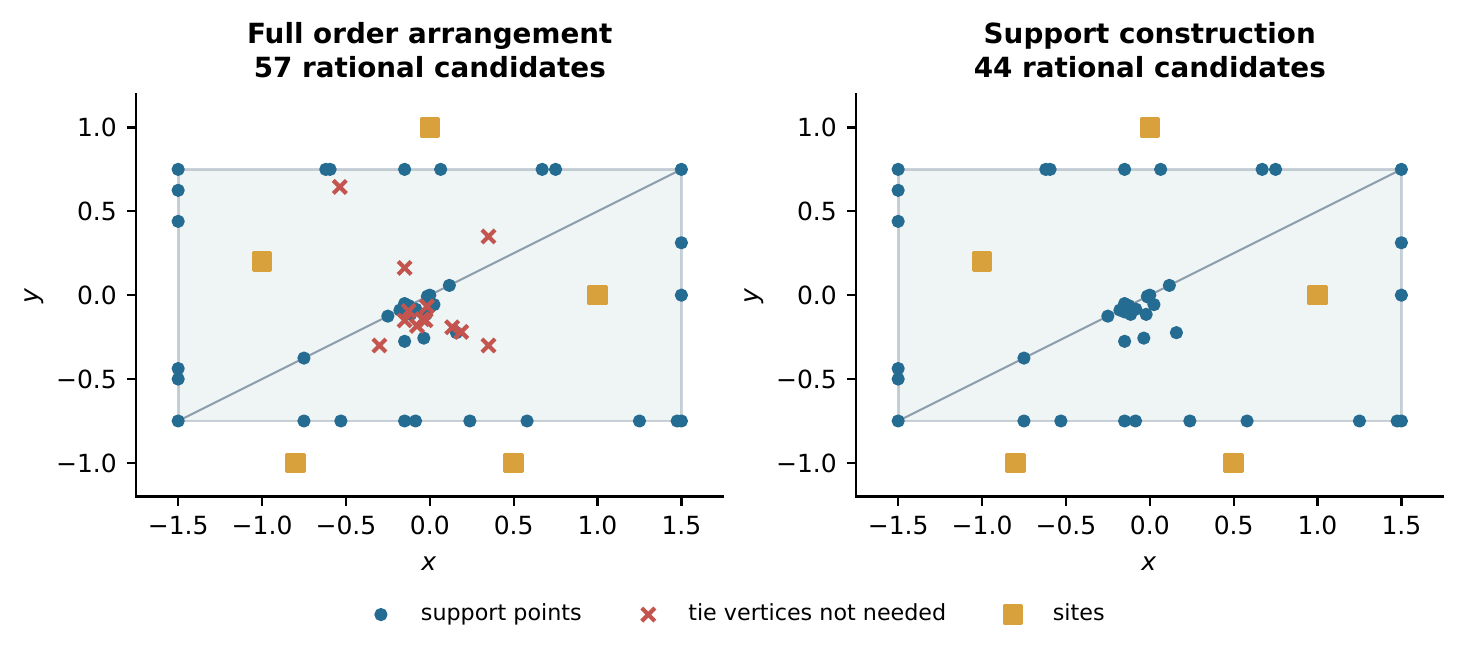
\includegraphics[width=\textwidth]{figures/support-comparison.png}
\caption{Two support constructions for five sites (gold squares) on the same two-triangle target. Left: the full distance-order arrangement, $57$ candidate points. Right: the support set of \cref{thm:support-radius}, $44$ points, valid for every monotone rule; the red crosses mark tie points of the arrangement that it does not need.}
\end{figure*}

\begin{figure*}[tb]
\centering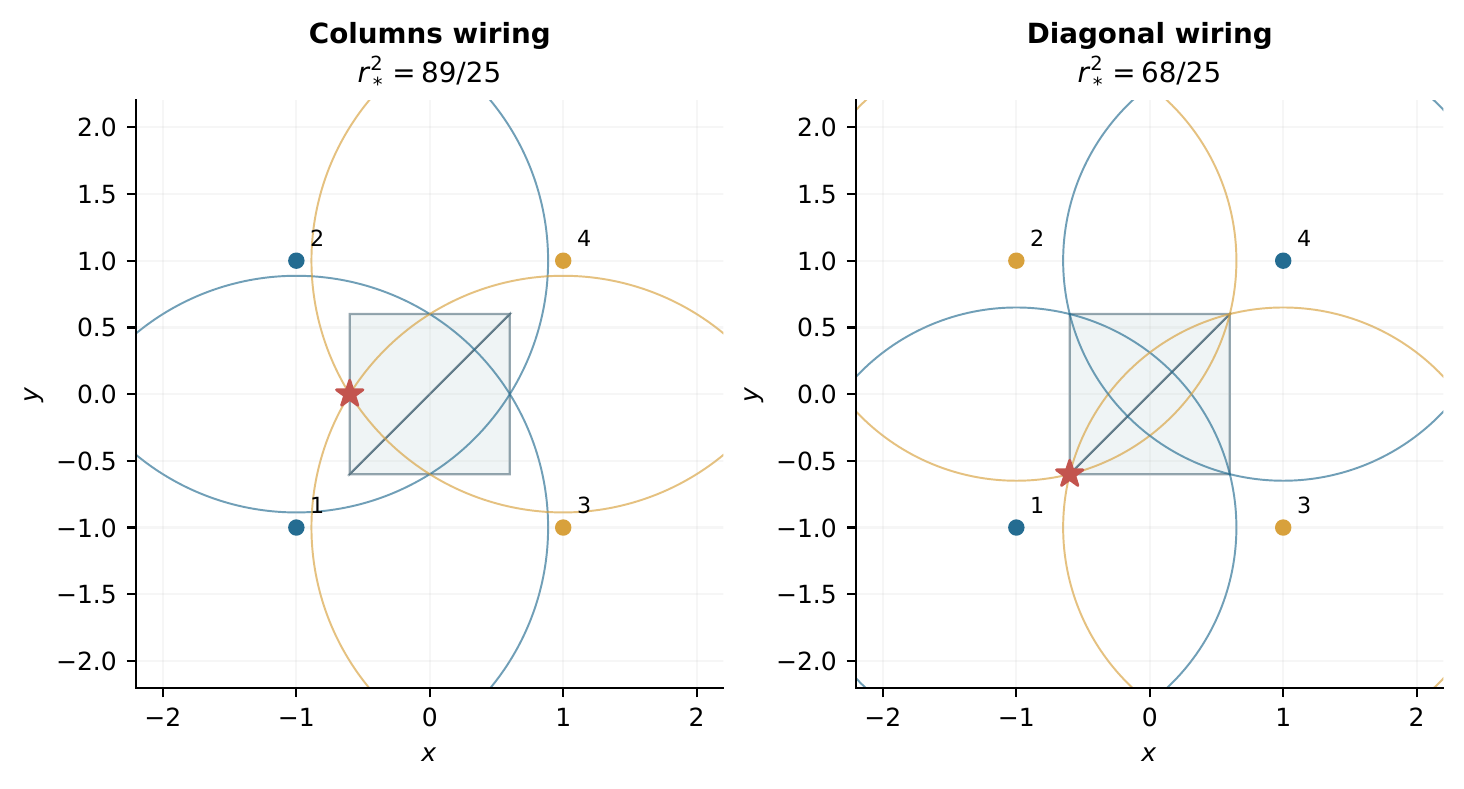
\includegraphics[width=\textwidth]{figures/radius-supports.png}
\caption{Exact critical-radius witnesses for the two wiring choices. Stars mark maximizing target locations. The circles are drawn at the certified threshold radii, whose squares are rational.}
\end{figure*}

